\documentclass[10pt,twocolumn]{article}

% use the oxycomps style file
\usepackage{oxycomps}
\usepackage{float}

\pdfinfo{
    /Title (Tutorial Report)
    /Author (Oliver Wilkins)
}

% set the title and author information
\title{Tutorial Report}
\author{Oliver Wilkins}
\affiliation{Occidental College}
\email{wilkins@oxy.edu}

\begin{document}

\maketitle

\section{Introduction}

My current thinking with regards to my Comps is to use simulation techniques to estimate of the loss aversion coefficient A, which measures the degree to which people psychologically ‘overweight’ losses relative to gains. There is a large literature in both economics and psychology around finding empirical estimations of A, with most estimates falling between 1 and 4. This relatively large range can be explained partially by the fact that many estimates are made by conducting a single study and backing out what the participant’s loss aversion coefficient must have been given that they made the decisions they did. The estimate obtained is therefore highly dependent on the context of the specific study and the makeup of its participants. Additionally, many of the studies rely on asking participants hypothetical questions, which may elicit unrealistic answers due to the lack of stakes involved.

To address the concerns described above, my plan is to model various large-scale systems which are influenced by loss aversion, such as the stock market, insurance markets, and savings behavior. I will then run simulations in which the participants in these systems have varying levels of loss aversion, which will be normally distributed with different means and standard deviations for each run, and choose as my estimate the one which produces results most consistent with empirical evidence across the various systems. My hope is this approach will generate an estimate most reflective of the entire population (at least within the west) given the scale and diversity of the systems modeled.

The tutorial I chose is relevant to my Comps topic in that it models a system and then runs it using various inputs in a ‘guess and check’ system in order to determine which input is best. In the tutorial, the system being modeled is a theater business, and the question it is answering is the optimal numbers of various types of staff to hire in order to keep wait times at a reasonable level. A successful outcome would be finding the minimum numbers of staff needed such that wait times are kept under 10 minutes, thereby minimizing costs such while maintaining a sufficient level of performance.


\section{Methods}

I completed the tutorial in the Jupyter notebook environment, using python and relying on the simpy package.

The steps of the tutorial can be classified into two main processes: setting up the framework of the simulation, then iteratively running it with varying inputs to determine the best ones. The tutorial is primarily focused on the first of these and provides no guidance on the second other than instructing the user to manually guess and check different inputs until they find a solution. I deviated only slightly from the tutorial in setting up the simulation framework. Given that my comps will require checking many inputs and that each run of the simulation will likely take a non-negligible amount of time, I chose to automate the process of finding the ‘best’ input solution, which represents a significant deviation from the tutorial.


\subsection{Simulation Framework}

Setting up the simulation framework began by defining the processes which make up the workings of the theater being simulated. There were three: selling tickets (done by cashiers), selling food (done by servers), and checking tickets (done by ushers). Each process took time, which was constant for selling and checking tickets and determined randomly within some range for selling food. If there were not any of the correct type of employee available when one of the services was needed, a line would form in a first in first out fashion. Defining the behavior of moviegoers was next. All moviegoers had to buy a ticket and have it checked, and with a 50\% probability chose to buy food. They also had an arrival time, which were distributed randomly over a set interval. The time each moviegoer took from arrival to when their ticket was finished being checked was tracked. 

Once the theater processes and moviegoer behavior were set up, the simulation could be run. For a given run, a set of moviegoers were created and assigned to arrival times and food-buying statuses. The theater was given the chosen number of each employee, and time began. The simulation finished once the last moviegoer had their ticket checked, and the average total wait time was computed. 

The only change I made to this section of the tutorial was to make the number of moviegoers in each run of the simulation fixed, as opposed to being random within some range. While it makes sense in the context of making management decisions about a movie theater to include variability in the number of patrons because that is reflective of reality, I am using simulation for a somewhat different purpose in my Comps. I am interested in the effect on systems of changing a single variable, and in order for the input testing (discussed in the next section) to be similar to how I will do it for my Comps any randomness within the model must occur enough times that any aggregate statistics about the agents within the simulation must be close to identical across different runs. Therefore, random decisions about arrival time or food preferences are okay because they occur many times, but a single random decision about the number of moviegoers is not. 

\subsection{Input Testing}

The tutorial had users test numbers of employees manually. This was practical since running the simulation took negligible time, and it was easy to get a feel for which type of employee was slowing down the theater's operations the most at any given point. I was able to get a solution which would be acceptable to the hypothetical manager of this theater within a couple minutes. However, this type of input testing approach likely would not work well for my Comps. I therefore deviated from the tutorial and wrote an automated input testing system. 

The testing system answered two questions. The first was the same as the goal of the tutorial: to find the minimum numbers of employees needed to achieve sub-ten minute wait times. The second was to to rank each employee by their marginal time savings, i.e. the amount of time saved relative to having one fewer employee. This would be useful to a hypothetical theater manager because if they could calculate the marginal benefit of a one minute shorter wait time, via survey techniques or otherwise, they could hire employees up to the point that marginal benefit equals marginal cost (the wage of the employee). Such a technique is profit-maximizing by definition. 

To answer the first question, I used a brute-force technique. I ran the simulation with every permutation of employee counts between 1 and 10 (numbers chosen based on my intuition from playing around with manual inputs), and chose the permutation with the fewest total employees that was under 10 minutes. 

To answer the second, I used the following algorithm. Run the simulation with one of each employee. Then, run the simulation three times with one more of each of the types (once with 2 cashiers, 1 server, 1 usher, once with 1, 2, 1, of the respective types, and once with 1, 1, 2). Determine which employee gives the most time gains relative to the initial run. Whichever one that is gets 'hired,' and included in the baseline for the next test. Repeat this process until 40 employees have been 'hired,' recording the time gains of each one. 

\section{Metrics and Results}

The goal of building a simulation capable of finding the optimal number of employees to handle was achieved. The first metric by which it was achieved is that the simulation found the minimum number of employees needed to keep wait times under 10 minutes. The number turned out to be 16, with the distribution across employee types being 9 cashiers, 6 servers, and 1 usher. This result makes intuitive sense given the amount of time that the tasks of the respective employees take taken as well as the proportion of moviegoers who use each of their services. 

The second metric by which the goal was achieved was via a calculation of each of the first 40 employee's marginal wait time savings benefit, assuming the most productive type of employee was chosen at every hiring decision. The charts below show the results of this calculation. The first is the total time by number of employees, which is included to help build context (including for the first metric). The second chart shows the marginal time savings by employee. If the hypothetical theater manager were to figure out the value of a minute of wait time savings, they could determine the optimal number of employees to hire by multiplying the y axis of the graph by the salary of an employee and finding which employee number corresponds to that value on the graph (again assuming the correct types are hired). 
\begin{figure}[H]
    \centering
    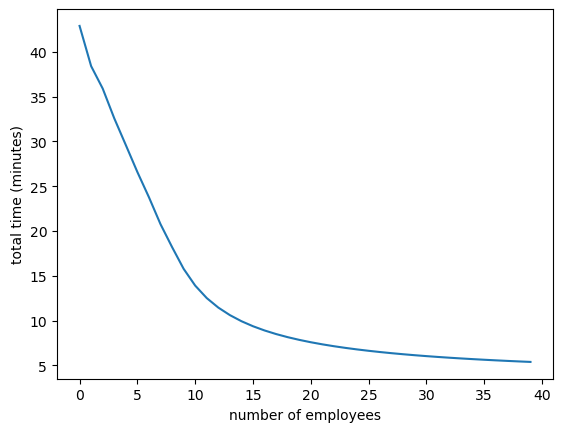
\includegraphics[width=0.9\linewidth]{totals.png}
    \caption{Total Time by Number of Employees}
    \label{fig:enter-label}
\end{figure}

\begin{figure}[H]
    \centering
    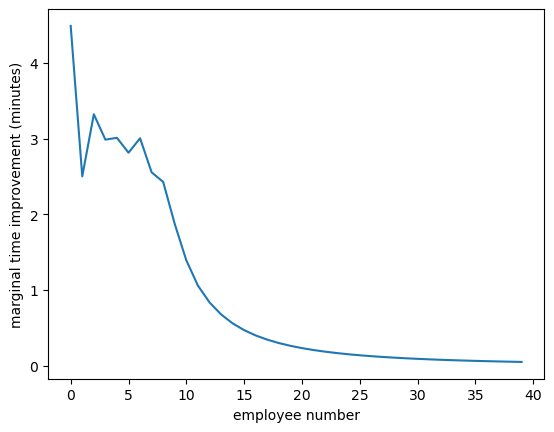
\includegraphics[width=0.9\linewidth]{marginal.png}
    \caption{Marginal Time Savings by Employee}
    \label{fig:enter-label}
\end{figure}

The degree to which the results of this simulation can be used to guide practical decisions speaks to the power of simulation as a tool, assuming the assumptions it makes are accurate. 

\section{Reflection}

Completing this tutorial has given me confidence that my knowledge of specific softwares, programming languages, or libraries will not be a limiting factor in my Comps, since I expect the same tools used in the tutorial would be sufficient for my Comps project. 

I still have concerns related to the algorithmic decisions I will have to make. In particular, the systems I am modeling are large and complex, and will need to be simplified significantly. Doing so in such a way that my results are not biased will require careful thinking and research. Another concern I have relates to creating a metric to measure how good each of my estimations of the loss aversion coefficient are. There are many empirical values that I will have to choose from and aggregate together. Doing so will require subjective judgements, and again I will have to be cautious so as not to bias my estimate.
\end{document}
